\documentclass[a4paper]{article}

\usepackage{tecnico_relatorio}

\usepackage{textcomp}
\usepackage[hypcap]{caption} % makes \ref point to top of figures and tables

\begin{document}
	\trSetImage{img/tecnico_logo}{6cm} % Logotipo do Técnico
	\trSetSubject{Arquitecturas Avançadas de Computadores}
	\trSetType{Laboratório I}
	\trSetTitle{Simulação de um Microprocessador \textmu RISC com Funcionamento Multi-ciclo}
	
	\trSetBoxStyle{0.3}
	
	\trSetAuthorNr{3}
	
	\trSetAuthors
		{
		Gonçalo Ribeiro
		
		73294
		}{
		Miguel Costa
		
		73359
		}{
		Rafael Gonçalves
		
		73786
		}
	
	
	\trMakeCover
	
	\tableofcontents
	\pagebreak
	
	\section{Introdução}
	
		Nesta actividade laboratorial pretende-se desenvolver um processador \textmu RISC com descrição em VHDL. Pretende-se que este processador com arquitectura RISC de 16 bits e funcionamento multi-ciclo execute 42 instruções diferentes, demorando 4 ciclos para completar cada uma. No primeiro ciclo (Instruction Fetch--IF), a próxima instrução a ser executada é carregada da memória e armazenada no registo de instruções. No segundo ciclo (Instruction Decode--ID) a instrução anteriormente carregada é descodificada e os operandos são lidos do Register File (RF). O terceiro ciclo (Execution--EX) consiste na execução da instrução e cálculo das condições dos resultados. Por fim, no quarto ciclo (Write Back--WB) os resultados são escritos no RF.
	
		Tal como já foi referido, é um processador de 16 bits que contém 8 registos de uso geral, cada um com 16 bits de largura. Existem 42 instruções possíveis de executar, sendo estas compostas por até 3 operandos. Quanto à memória esta é do tipo big endian, sendo endereçável ao nível da palavra.
	
	
	\section{Arquitectura}
	
		\subsection{IF}

			\begin{figure}[H]
				\centering	
				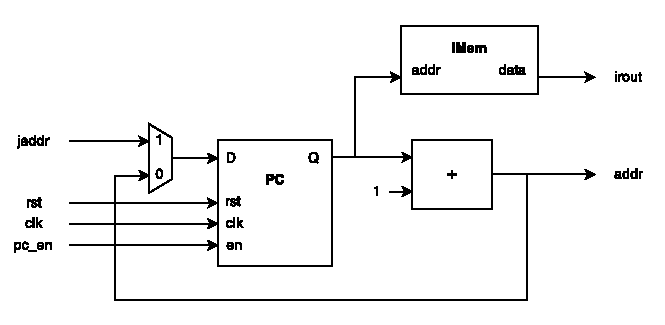
\includegraphics[width=1.\textwidth]{img/IF}
				\caption{Bloco \textit{Instruction Fetch}--IF}
				\label{fig:if}
			\end{figure}

			A unidade \textit{Instruction Fetch} (IF) mantém o registo de qual a instrução do programa que está a ser correntemente executada. As suas saídas são a instrução actual e o endereço da próxima instrução. O IF é também responsável por actualizar o PC a cada flanco de relógio de forma a passar para a instrução seguinte. Ou, no caso de instruções de salto (\texttt{jump}), é responsável por actualizar o PC de forma a que a próxima instrução corresponda ao endereço se salto pretendido.
			
			O esquema do IF pode ser visto na \autoref{fig:if}. A descrição deste componente encontra-se no ficheiro \texttt{IF.vhd}.

			\subsubsection{PC}

			O \textit{Program Counter} (PC) é um contador que em cada momento contém o endereço da memória em que se encontra a instrução a executar. No caso de instruções ``normais'' o valor do PC é incrementado em uma unidade. No caso de instruções de salto o PC suporta o carregamento de um ponteiro para a próxima instrução que deve ser executada.
			
			Quando o \textmu RISC é iniciado a primeira instrução que deve ser executada é a que se encontra no endereço 0 da memória de programa. Assim sendo, o PC conta com um sinal de resete (\texttt{rst}) que é usado para que o valor do PC seja 0 no inicio da execução.

			\subsubsection{ROM}

			No caso do \textmu RISC optou-se por usar uma ROM como memória de programa. Esta ROM é endereçada à palavra (16 bits), constituindo cada palavra uma instrução do programa. A ROM é um bloco assíncrono de forma a que mal seja endereçada a instrução seja propagada para a saída. Se ROM fosse síncrona seria necessário esperar até o final do ciclo de relógio para obter a instrução.
			
			A ROM utilizada tem 16k palavras. Como o PC tem 16 bits seria possível expandir a ROM até 64k palavras. Criou-se a ROM de forma a que o XST leia um ficheiro de texto que contém as palavras a colocar na mesma. Desta forma, basta fornecer diferentes ficheiros ao XST para que a ROM seja inicializada com diferentes programas.
			
			A descrição da ROM pode encontrar-se no ficheiro \texttt{IMem.vhd}.


		\subsection{IDRF}
			
			
			
			
			
			\subsubsection{RF}
			
		\subsection{EX}
		
			\begin{figure}[H]
				\centering
				\centerline{
					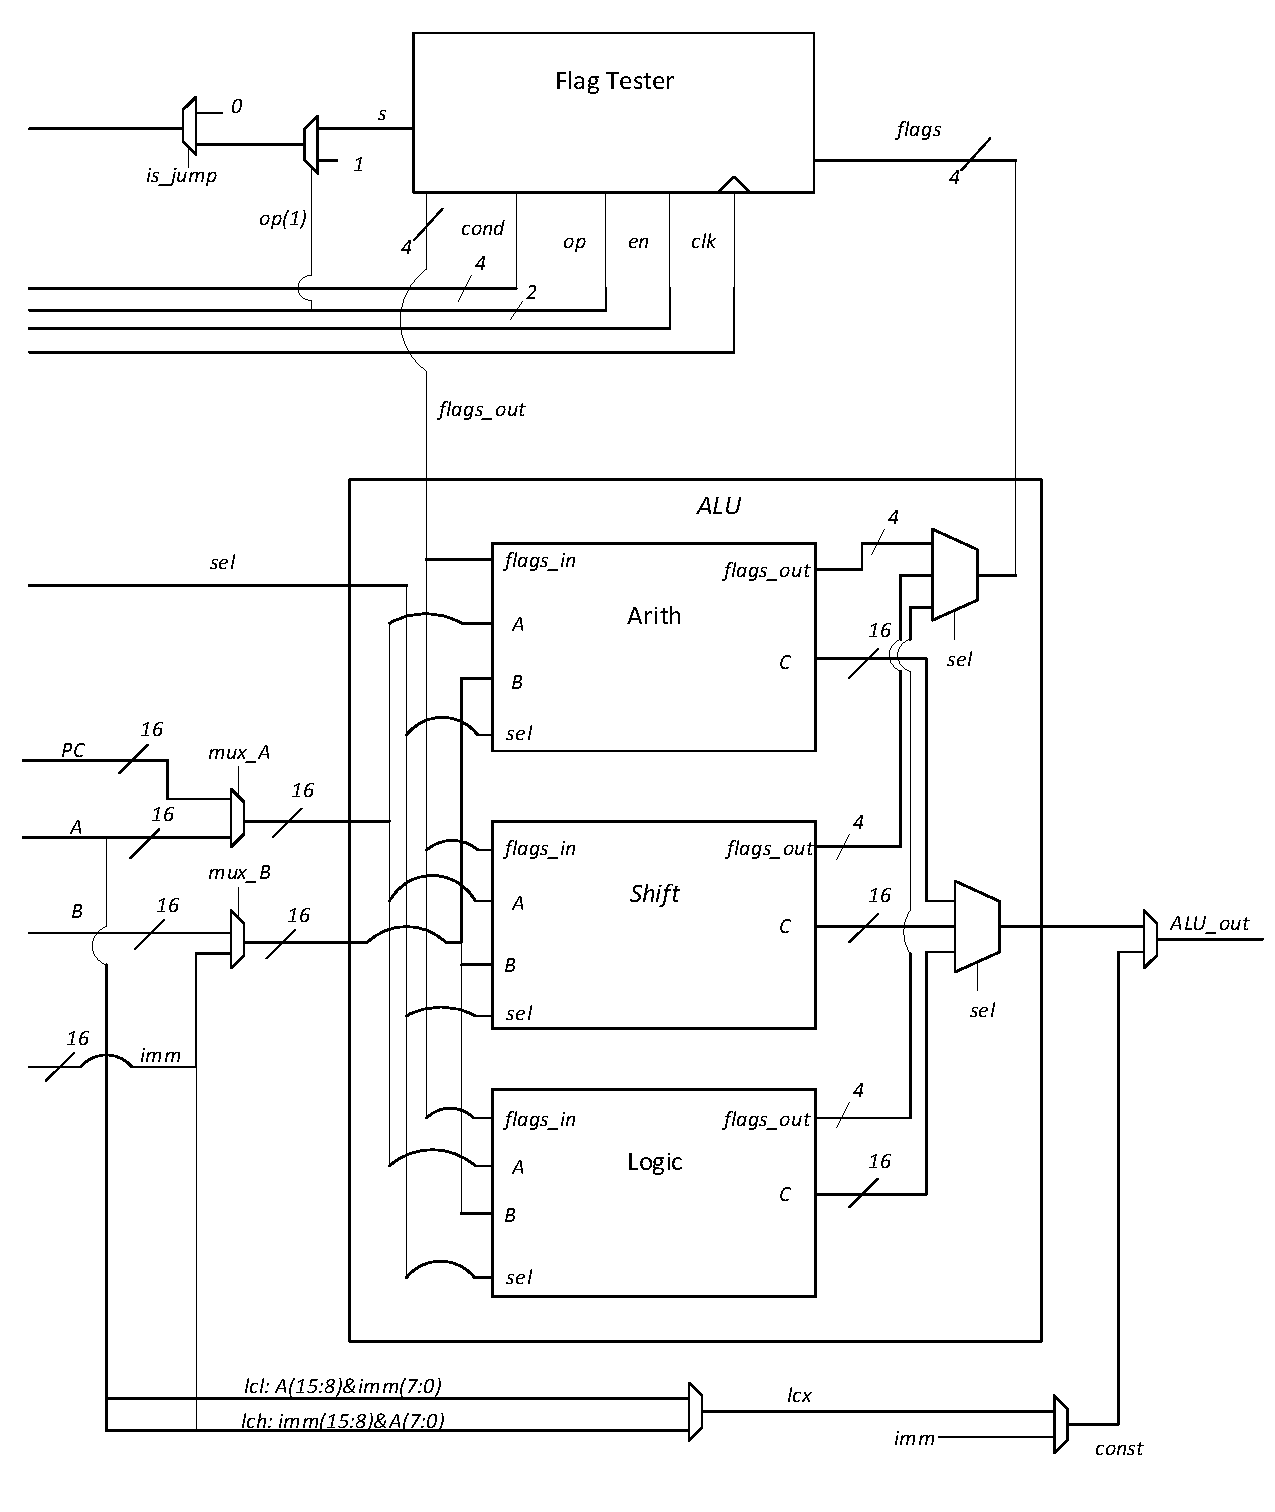
\includegraphics[width=.8\paperwidth]{img/EX}
				}
				\caption{Bloco de Execução e acesso à memória--EX/MEM}
				\label{fig:ex}
			\end{figure}
		
			Neste módulo são executadas as instruções e calculadas as condições de resultados. Podemos então considerar 3 grandes componentes que funcionam neste ciclo: ALU, Flag Tester e RAM.
			
			Tal como é visível na \autoref{fig:ex}, podemos ainda considerar lógica adicional, correspondente ao \textit{load} de constantes. Como o processador permite o carregamento de constantes para a parte \textit{high} ou parte \textit{low}, é feita aqui essa concatenação, sendo que depois é feita uma multiplexagem para os restantes casos de carregamento de constantes (que provêm do \textit{Signal Extender} em IDRF).
		
			\subsubsection{ALU}
				
				O componente da ALU é responsável por receber 2 operandos ($A$ e $B$), efectuar uma dada operação sobre estes (aritmética, deslocamento lógico ou lógica), dando um resultado $C$.
				
				Este componente é divisível em 3 subcomponentes: componente aritmética, lógica e shifts. É neste componente que são geradas as \textit{flags}, consoante a operação a executar. Existem então 4 \textit{flags}: \textit{signal} ($S$), \textit{carry} ($C$), \textit{zero} ($Z$) e \textit{overflow} ($V$). Mais à frente são descritas as funcionalidades destas e quais as suas utilidades.
				
				O primeiro sub-componente é responsável por executar qualquer função aritmética: soma, subtração e as suas variantes. É de notar que nestas operações todas as \textit{flags} são actualizadas neste bloco.
				
				O componente responsável por fazer os deslocamentos lógicos (shifts) apenas tem que efectuar duas operações: shift aritmético direito e shift lógico esquerdo. Neste bloco são actualizadas as \textit{flags} de signal, zero e carry.
				
				Por último, a unidade lógica é responsável por efectuar todas as operações lógicas: \texttt{and}, \texttt{or}, \texttt{xor}, \texttt{pass}, \texttt{nor}, \texttt{nand}, entre outras. Neste componente, por a actualização das \textit{flags} ser independente de operação para operação, é apenas feita a actualização das que forem necessárias (zero, signal ou nenhuma).
			
			\subsubsection{RAM}
				
				O bloco de memória RAM, tal como já foi referido, é endereçável ao nível da palavra, sendo que cada endereço de memória corresponde então a uma palavra de 2 bytes. Se o processador tem 16 bits de endereço, então a capacidade total de memória do processador é de 32 kB. Esta memória funciona com leitura assíncrona e escrita síncrona caso o enable de escrita se encontre activo (\texttt{we = '1'}).
				
				Quanto à descrição VHDL, a memória tem como sinal de entrada \texttt{data\_in}, de saída \texttt{data\_out} e de endereço \texttt{addr}, ou seja, para as instruções existentes de acesso à memória temos que podem ser feitas as operações de \texttt{load} e \texttt{store}. Quanto à primeira é carregado para um registo $C$ o valor da memória endereçável pelo conteúdo do registo $A$; quanto à segunda instrução é armazenado o conteúdo do registo $B$ no endereço de memória apontado pelo conteúdo do registo $A$.
				
			\subsubsection{Flag Tester}
			
				Quanto à actualização das \textit{flags}, tal como já foi referido, o método utilizado baseia-se em actualizar apenas as \textit{flags} necessárias, ou seja, todas as \textit{flags} guardadas entram dentro da ALU, mas dependendo da instrução a executar, é feita uma concatenação das \textit{flags} a actualizar com as que não serão actualizadas. No entanto, no caso de ser uma operação aritmética, todas as \textit{flags} são actualizadas.
			
				O componente de Flag Tester serve então para indicar se se deve efectuar um determinado salto ou não dependendo se é instrução de salto ou se as condições de flag são válidas para que se efectue esse salto. Temos então como sinais de entrada as quatro \textit{flags}, o código correspondente à condição de salto, o código da operação a efectuar (para distinguir os vários tipos de salto), um \textit{enable} e como sinais de saída os valores das \textit{flags} armazendos em registos e ainda um sinal \texttt{s} que indica qual valor de PC a utilizar, se PC+1 ou se um outro valor de PC. Em primeiro lugar é verificada a condição de salto de acordo com os sinais presentes nos registos das \textit{flags}, a operação de salto, e caso se verifique que a condição é verdadeira para o salto indicado, então é colocado \texttt{s} com valor lógico `1'. Caso a condição não seja cumprida, é colocado o valor lógico `0'. 
				
				À saída deste bloco temos ainda lógica adicional para indicar caso não seja uma operação de salto (\textit{mux} regulado por \texttt{is\_jump}), sendo que se for um \texttt{jump true} ou \texttt{jump false}, é enviado o sinal proveniente do \emph{Flag Tester}, mas caso seja um outro tipo de salto (salto incondicional, por exemplo), seja carregado na mesma o valor do salto e não PC+1.
			
				
		\subsection{WB}
		
			\begin{figure}[H]
				\centering
				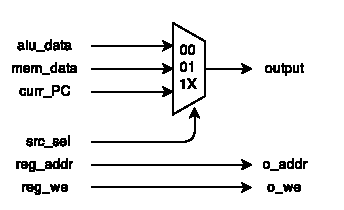
\includegraphics[width=.8\textwidth]{img/WB}
				\caption{Bloco \textit{Write-Back}--WB}
				\label{fig:wb}
			\end{figure}
			
			O bloco \textit{Write-Back} (WB) é o mais simples do \textmu RISC. É constituído por um multiplexer que deixa passar um de três sinais: o resultado proveniente da ALU; ou uma palavra da memória; ou o valor de PC+1. O resultado da ALU é deixado passar no caso de operações que usam a ALU; a palavra de memória passa no caso das instruções de \texttt{load}; e PC+1 é usado para a instrução \texttt{jal}, em que o valor do PC é carregado para um registo (o registo R7).
			
			O valor que passa para a saída \texttt{output} só é relevante para as operações que actualizam os registos do \textit{Register File}. Pelo WB passam também os sinais que permitem endereçar o RF e o sinal de enable do mesmo.
			
			O esquema do WB está patente na \autoref{fig:wb} e o ficheiro que o descreve é o \texttt{WB.vdh}.
			

		\subsection{Máquina de Estados}
		
			\begin{figure}[H]
				\centering
				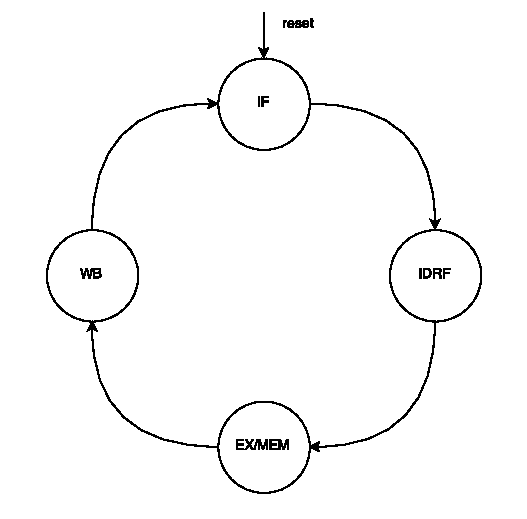
\includegraphics[width=.8\textwidth]{img/maqestados}
				\caption{Máquina de Estados que regula os enables dos andares de registos}
				\label{fig:maqestados}
			\end{figure}
		
			De maneira a sincronizar os andares de registos dos vários módulos, foi adicionada uma Máquina de Estados de Moore muito simples, com quatro estados sequenciais consecutivos, cada um correspondente a um dos andares do microprocessador (ver \autoref{fig:maquestados}).
		
	\section{Testes e Simulações}
	
		Para testar o \textmu RISC foram utilizados vários programas escritos em \textit{assembly}. Alguns programas foram fornecidos pelo professor, nomeadamente um que calcula os primeiros 20 números da sequência da Fibonnacci (\autoref{subsec:sim_fib}). Outros foram escritos pelo grupo. Entre estes últimos encontra-se um teste que incide sobre \textit{jumps}, outro sobre \textit{flags}, outro sobre \textit{shifts} e um último sobre \textit{overflows}.
		
		Todos os testes utilizados para testar o \textmu RISC bem como \textit{scripts} usados para converter o resultado do \textit{linker} para o formato lido pelo XST para inicializar a ROM encontram-se na pasta \texttt{asm} entregue em conjunto com o presente relatório.
	
		\subsection{Fibonacci}
		\label{subsec:sim_fib}
		
	\section{Conclusão}

	\bibliographystyle{plain}
	\nocite{xilinx}
	\bibliography{xilinx}	% no spaces between commas!

\end{document}
